%  LaTeX support: latex@mdpi.com
%  In case you need support, please attach any log files that you could have, and specify the details of your LaTeX setup (which operating system and LaTeX version / tools you are using).

%=================================================================

% LaTeX Class File and Rendering Mode (choose one)
% You will need to save the "mdpi.cls" and "mdpi.bst" files into the same folder as this template file.

%=================================================================

\documentclass[atoms,article,submit,moreauthors,pdftex,12pt,a4paper]{mdpi} 
%--------------------
% Class Options:
%--------------------
% journal
%----------
% Choose between the following MDPI journals:
% actuators, administrativesciences, aerospace, agriculture, agronomy, algorithms, animals, antibiotics, antibodies, antioxidants, appliedsciences, arts, atmosphere, atoms, axioms, batteries, behavioralsciences, bioengineering, biology, biomedicines, biomolecules, biosensors, brainsciences, buildings, cancers, catalysts, cells, challenges, chemosensors, children, chromatography, climate, coatings, computation, computers, cosmetics, crystals, dentistryjournal, diagnostics, diseases, diversity, econometrics, economies, education, electronics, energies, entropy, environmentalsciences, environments, epigenomes, fibers, foods, forests, futureinternet, galaxies, games, gels, genealogy, genes, geosciences, healthcare, horticulturae, humanities, hydrology, informatics, information, inorganics, insects, ijerph, ijfs, ijms, ijgi, jcdd, jcm, jdb, jfb, jimaging, jof, joi, jlpea, jmse, jpm, jrfm, jsan, land, laws, life, lubricants, machines, marinedrugs, materials, mathematics, medicalsciences, membranes, metabolites, metals, microarrays, micromachines, microorganisms, minerals, molbank, molecules, nanomaterials, ncrna, nutrients, pathogens, pharmaceuticals, pharmaceutics, pharmacy, photonics, plants, polymers, processes, proteomes, publications, religions, remotesensing, resources, risks, robotics, safety, sensors, sinusitis, socialsciences, societies, sports, standards, sustainability, symmetry, systems, technologies, toxics, toxins, universe, vaccines, veterinarysciences, viruses, water
%---------
% article
%---------
% The default type of manuscript is article, but could be replaced by using one of the class options: 
% article, review, communication, commentary, bookreview, correction, addendum, editorial, changes, supfile, casereport, comment, conceptpaper, conferencereport, meetingreport, discussion, essay, letter, newbookreceived, opinion, projectreport, reply, retraction, shortnote, technicalnote, creative
%----------
% submit
%----------
% The class option "submit" will be changed to "accept" by the Editorial Office when the paper is accepted. This will only make changes to the frontpage (e.g. the logo of the journal will get visible), the headings, and the copyright information. Journal info and pagination for accepted papers will also be assigned by the Editorial Office.
% Please insert a blank line is before and after all equation and eqnarray environments to ensure proper line numbering when option submit is chosen
%------------------
% moreauthors
%------------------
% If there is only one author the class option oneauthor should be used. Otherwise use the class option moreauthors.
%---------
% pdftex
%---------
% The option "pdftex" is for use with pdfLaTeX only. If eps figure are used, use the optioin "dvipdfm", with LaTeX and dvi2pdf only.

%=================================================================
\setcounter{page}{1}
\lastpage{x}
\doinum{10.3390/------}
\pubvolume{xx}
\pubyear{2015}
%\externaleditor{Academic Editor: xx}
\history{Received: xx / Accepted: xx / Published: xx}
%------------------------------------------------------------------
% The following line should be uncommented if the LaTeX file is uploaded to arXiv.org
%\pdfoutput=1

%=================================================================

% Add packages and commands to include here
% The amsmath, amsthm, amssymb, hyperref, caption, float and color packages are loaded by the MDPI class.
\usepackage{graphicx}
\usepackage{color}
%\usepackage{subfigure,psfig}

%=================================================================
%% Please use the following mathematics environments:
%\theoremstyle{mdpi}
%\newcounter{thm}
%\setcounter{thm}{0}
%\newcounter{ex}
%\setcounter{ex}{0}
%\newcounter{re}
%\setcounter{re}{0}
%\newtheorem{Theorem}[thm]{Theorem}
%\newtheorem{Lemma}[thm]{Lemma}
%\newtheorem{Characterization}[thm]{Characterization}
%\newtheorem{Proposition}[thm]{Proposition}
%\newtheorem{Property}[thm]{Property}
%\newtheorem{Problem}[thm]{Problem}
%\newtheorem{Example}[ex]{Example}
%\newtheorem{Remark}[re]{Remark}
%\newtheorem{Corollary}[thm]{Corollary}
%\newtheorem{Definition}[thm]{Definition}
%% For proofs, please use the proof environment (the amsthm package is loaded by the MDPI class).

%=================================================================
\def\be{\begin{equation}}
\def\ee{\end{equation}}
\def\ba{\begin{eqnarray}}
\def\ea{\end{eqnarray}}

% Full title of the paper (Capitalized)
\Title{Cavity-Assisted Spin-Orbit Coupling of Ultracold atoms}

% Authors (Add full first names)
\Author{Lin Dong $^{1,}$, Chuanzhou Zhu $^{1}$ and Han Pu $^{1}$*}

% Affiliations / Addresses (Add [1] after \address if there is only one affiliation.)
\address{%
$^{1}$ Department of Physics and Astronomy, Rice Quantum Institute, Rice University, Houston, Texas, 77251-1892, USA
}


% Contact information of the corresponding author (Add [2] after \corres if there are more than one corresponding author.)
\corres{hpu@rice.edu}

% Abstract (Do not use inserted blank lines, i.e. \\) 
\abstract{We investigate dynamical and static properties of ultracold atoms confined in an optical cavity, where two photon Raman process induces effective coupling between atom's pseudo-spin and center-of-mass momentum. In the meantime, atomic dynamics exerts a back action to cavity photons. We adopt both mean field and master equation approach to tackle the problem and found surprising modifications to atomic dispersions and dynamical instabilities, arising from the intrinsic nonlinearity of the system. Correspondence between semi-classical and quantum limits is analyzed as well.}

% Keywords: add 3 to 10 keywords
\keyword{cavity quantum electrodynamics; cold atoms; spin-orbit coupling}

% The fields PACS, MSC, and JEL may be left empty or commented out if not applicable
%\PACS{}
%\MSC{}
%\JEL{}

% If this is an expanded version of a conference paper, please cite it here: enter the full citation of your conference paper, and add $^\dagger$ in the end of the title of this article.
%\conference{}

\begin{document}

%%%%%%%%%%%%%%%%%%%%%%%%%%%%%%%%%%%%%%%%%%

\section{Introduction}
%%%%%%%%%%%%%%%%%%%%%%%%%%%%%%%%%%%%%%%%%%
%\subsection{This is a Subsection Heading}
%%%%%%%%%%%%%%%%%%%%%%%%%%%%%%%%%%%%%%%%%%

% Main text paragraph. Citing a journal paper \cite{ref-journal}. And now citing a book reference \cite{ref-book}.
%Laser light is a versatile and {\em de facto} standard experimental tool in the forefront field of modern quantum optics and ultracold atomic gases. Spatial coherence allows a laser beam to be focused to a tight spot and stay narrow over long distances. Extremely narrow energy spectrum, given by high temporal coherence, makes it ideal to create highly controllable and tunable optical potentials, when far red detuned from an atomic resonances. The pioneering experimental achievement of Bose-Einstein condensation (BEC) \cite{BEC1, BEC2, BEC3}, and of Fermi degenerate dilute gases \cite{Fermi1, Fermi2, Fermi3} has offered a plethora of opportunities to study quantum properties of light and ultracold matter. A major focus in recent years has been the exploration of quantum properties of many-body strongly correlated systems (for reviews, cf \cite{Bloch1, Bloch2}) , by trapping coherent matter waves in optical potentials, e.g. harmonic trap, optical lattices, etc. A high level of microscopic understanding sheds light on some of long sought problems in condensed matter and high energy physics, e.g. Bose-Hubbard (BH) model \cite{BH1, BH2}, universal physics of strongly interacting fermions \cite{Fermi4, Fermi5}. However, quantum effects of the light were widely neglected to a large extent. In both complex experimental setups and theoretical models, laser light is commonly treated as a classical auxiliary tool to prepare, probe and manipulate intriguing atomic states. Atom-field interaction can be well captured by the minimal-coupling Hamiltonian at the dipole approximation level. In the far red detuned limit, coherent scattering of photon dominate and the resulting dipole light force can be derived from the optical potential proportional to laser intensities due to Stark-shift. 

Cavity quantum electrodynamics (CQED) was a field originally devoted to study the radiation effect of atoms when different geometric boundaries are present. Recent technological advancements in cavity further allows us to explore the so-called ``strong coupling regime'' in both microwave and optical frequency domains, where coherent scattering between an atomic transition and a single electromagnetic mode dominates over all dissipation processes.  When this ideal experimental tabletop is combined with  cold atoms \cite{cavity1, cavity2, cavity3}, atoms and the light field will mutually affect each other. This is simply because intra-cavity photon and atoms very frequently scatter with each other due to the geometric confinement. Dipole force gets strongly enhanced and and atom's back-action {\em onto} light gets significant. In general, this demands a self-consistent solution for both light and atom by treating them on equal footing. On the one hand, the quantum properties of atom will manifest themselves in the scattered light, which leads to novel technical advancements in probing atomic states using light. On the other hand, the quantized light field imprints nontrivial marks on atomic many-body dynamics as well as equilibrium states. In this regard, cavity quantum electrodynamics (CQED) further enriches the picture of quantum simulations \cite{cavity4, cavity5, cavity6}. Although in the dispersive regime of CQED, where the resonant exchange energy between atom and field is strongly suppressed due to large detuning, the position-dependent cavity frequency shift exceeds the cavity linewidth. The center-of-mass (COM) motion of the atom becomes non-negligible in this ``ultracold atom + optical cavity'' system, which has been extensively explored both experimentally \cite{cavity7, cavity8, cavity9, cavity10, cavity11} and theoretically \cite{cavity12, cavity13}. 

Another series of breakthrough in cold atoms research stem from the recent realization of artificial (synthetic) gauge potentials for neutral atoms, first in bosonic systems \cite{soc1, soc2} and later in fermionic counterparts \cite{soc3, soc4}. Laser fields are properly aligned and designed in such a way that trapped atoms may mimic charged particles in a magnetic field with emergence of Lorentz-like force. The synthesis is achieved by inducing two-photon Raman transition between two hyperfine ground state. Using a group of degenerate (or quasi-degenerate) pseudospin eigenstates, non-abelian dynamics of cold atoms in light fields is generated, which effectively leads to the spin-orbit coupling (SOC) for cold atoms, simulating the one appearing for electrons in condensed matter. Synthetic SOC refers to the coupling between pseudospins (i.e. hyperfine states) and atom's COM motion, rather than the generic interaction between electron's spin (or magnetic moment) and angular/linear momentum operator in quantum mechanics. SOC is essential in understanding numerous underlying condensed matter phenomena and particle physics \cite{socVictor}, including {\em inter alia} topological insulators, Majorana and Weyl fermions, spin-Hall effects, etc \cite{TI, MF, WF, SHE1, SHE2}. 

Thus far, all the experimental realizations of synthetic SOC in quantum gases, utilize classical laser fields to assist Raman transition, which are not affected by atom's COM reciprocally. In this article of special issue, we first of all briefly review our previous work \cite{cavitySOC}, and theoretically explore the full quantum treatment beyond semi-classical mean field formalism, then investigate the correspondences in quantum and semi-classical regions. We consider a single atom (or an ensemble of $\mathcal{N}$ non-interacting  bosons) being confined by a single-mode unidirectional ring cavity, whose cavity mode together with an additional coherent laser beam form a pair of Raman beams that flips atomic transition between $|\uparrow\rangle$ and $|\downarrow\rangle$ while transferring recoil momentum of $\pm2\hbar q_r\hat{z}$ from and/or to photon field. Hence, the so-realized effective coupling between atom's external and internal degrees of freedom is generated by the quantized light field, which is affected by atomic dynamics in return. In this sense, the {\em cavity-assisted} SOC becomes {\em dynamic}. We show that, at mean field level, the dynamic SOC dramatically modifies the atomic dispersion relation, in particular, with emergence of a loop structure under certain circumstances. We systematically characterize dispersion relation of atomic state and photon number, both as a function of atom's quasi-momentum. For given cavity parameters, we found with increasing Raman coupling strength $\Omega$, dispersion curve changes from double minima to gapped single minimum, looped structure, and gapless single minimum in sequence. Furthermore, we carry out the full quantum mechanical treatment by solving master equations of density operators, and find excellent agreement by comparing averaged photon number with mean field results. The two distinctively different approaches give us an unified understanding of the atom-light effective non-linearity and induced dynamical instability in this system.

The article is organized as the following: After briefly reviewing key ideas of our previous work and semi-classical mean field approach in Sec. \ref{meanfield}, we develop the full quantum mechanical formalism to the physical system of interest in Sec. \ref{master} and discuss about the intimate correspondence between the two in Sec. \ref{relation}, and finally conclude in Sec. \ref{conclusion}. 

\section{Model Setup and Semi-classical Mean Field Formalism} \label{meanfield}

We follow the effective model Hamiltonian proposed in \cite{cavitySOC}, 
\ba
 \mathcal{H}_{\rm eff}& = & \sum_\sigma\int d{\bf r}\left[ \psi^\dagger_\sigma({\bf r})\left(\frac{ \hat{{\bf k}}^2+ 2\alpha q_r {k}_z}{2m}+\alpha\tilde{\delta}\right)\psi_\sigma({\bf r})\right]+  \frac{\Omega}{2}\int d{\bf r}\left[{\psi}_{\uparrow}^{\dagger}({\bf r}){\psi}_{\downarrow}({\bf r})c+ h.c. \right]\nonumber \\
 & + & i\varepsilon_{p}(c^{\dagger}-c)-\delta_c c^{\dagger}c-i\kappa c^{\dagger}c, \label{effH}
 \ea
where $\psi_\sigma({\bf r})$ ($\sigma = \uparrow$, $\downarrow$) is the atomic operator after gauge transformation in rotating frame at pump frequency $\omega_p$. $\alpha=\pm 1$ for $\sigma=\uparrow,\downarrow$, respectively. $q_r$ denotes recoil momentum, $\tilde{\delta}$ represents the two-photon Raman detuning, $\varepsilon_p$ refers to pumping rate, and $\delta_c$ is the cavity-pump detuning. $\Omega$ describes the atom-photon coupling strength, however, the entire Raman coupling term $ \frac{\Omega}{2}\int d{\bf r}e^{+2i k_{r}z}\Psi_{\uparrow}^{\dagger}({\bf r})\Psi_{\downarrow}({\bf r})\tilde{c}e^{+i\omega_{R}t}$ together with its hermitian conjugate describe cavity-assisted two-photon Raman transition processes, where cavity photon amplitude of $\tilde{c}$ or $\tilde{c}^\dag$ is explicitly taken into consideration. It is this coupling that renders the resulting SOC \emph{dynamic}. Furthermore, in the semi-classical approach, we have treated the leakage of cavity photon phenomenologically by introducing a cavity decay rate $\kappa$. 

From the Hamiltonian~(\ref{effH}), one can easily obtain the EOM in Heisenberg picture. To make some progress, we adopt a mean-field approximation by replacing the operators by their respective expectation values: $c \rightarrow \langle c \rangle \,, \psi_\sigma ({\bf r}) \rightarrow \langle \psi_\sigma ({\bf r}) \rangle \equiv \varphi_\sigma ({\bf r})$. 
%The mean-field approximation is justified by assuming small quantum fluctuations of both operators $c$ and $\psi_\sigma({\bf r})$. 
Assuming spatial homogeneity, we further take the plane-wave ansatz for the atomic modes $\varphi_\sigma({\bf r})=e^{i{\bf k}\cdot{\bf r}}\varphi_\sigma$ with the normalization condition $|\varphi_\uparrow|^2+|\varphi_\downarrow|^2=\mathcal{N}$. The steady-state solution for the photon field is obtained by taking the time derivative of the photon field to be zero, which is exact by itself without making further approximations %This is known as adiabatic elimination, which essentially assumes cavity photon can always follow atom's instantaneous eigenstates, typically valid for current high-Q cavity experiments. 
After some algebra, we write down the coupled nonlinear time-dependent equations for the two spin components, 
\ba
i\dot{\varphi}_{\uparrow}&\!\! =\!\! & \left(\frac{{\bf k}^{2}}{2m}+q_{r}k_{z}+\tilde{\delta}\right) \varphi_{\uparrow}+\frac{\Omega}{2}\frac{\varepsilon_{p}-\frac{i\Omega}{2} \mathcal{N}\varphi_\downarrow^\ast\varphi_\uparrow}{\kappa-i\delta_{c}}\varphi_{\downarrow} \,,\label{EOMphi1}\\
i\dot{\varphi}_{\downarrow} & \!\!= \!\!& \left(\frac{{\bf k}^{2}}{2m}-q_{r}k_{z}-\tilde{\delta}\right)\varphi_{\downarrow}+\frac{\Omega}{2}\frac{\varepsilon_{p}+\frac{i\Omega}{2} \mathcal{N}\varphi_\uparrow^\ast\varphi_\downarrow}{\kappa+i\delta_{c}}\varphi_{\uparrow}\,.\label{EOMphi2}
\ea

For a given atomic quasi-momentum ${\bf k}$, we define eigenstate and eigenenergy as the solution of the time-independent version of Eqs.~(\ref{EOMphi1}) and (\ref{EOMphi2}),  by replacing $i(\partial/\partial t)$ with $\epsilon({\bf k})$. After some lengthy nonetheless straightforward algebra, we find that $\epsilon({\bf k})$ obeys a quartic equation (we consider $\mathcal{N}=1$ hereafter): 
\begin{equation}
4\epsilon^4+B\epsilon^3+C\epsilon^2+D\epsilon+E=0 \,,
\label{generalquarticEq}
\end{equation}
where detailed derivations and coefficients are better elaborated in the Supplementary Material of \cite{cavitySOC}. 

[{\color{red} Rewrite it, simplify it and highlight it.}] In principle, the quartic equation~(\ref{generalquarticEq}) can be solved analytically, but the expressions too cumbersome to give any physical insights. We plot the typical behavior of the dispersion relation $\epsilon({ k_z})$ vs $k_z$ for $\tilde{\delta}=0$ in Fig.~\ref{atomloops}. Note that we always take $k_x =k_y=0$, as the SOC only occurs along the $z$-axis. A maximum of four real roots are allowed by Eq.~(\ref{generalquarticEq}). As we will show, in such regimes, a loop structure develops in the dispersion curve.
As shown in Fig.~\ref{atomloops}, for $\delta_c=0$ (i.e., the pump field is resonant with the cavity), we always have two dispersion branches. The two branches are gapped when the atom-photon coupling strength $\Omega$ is small and touch each other at $k_z=0$ when $\Omega$ exceeds a critical value. For $\delta_c \neq 0$, we again have two gapped branches at small $\Omega$. As $\Omega$ is increased beyond a critical value, a loop appears near $k_z=0$ in either the upper or the lower branch depending on the sign of $\delta_c$. The loop increases in size as $\Omega$ increases and finally touches the other branch and dissolves when $\Omega$ reaches a second critical value. Note that such a dispersion relation is markedly different from that without the cavity, in which case one always obtains two gapped branches. The dispersion curves for finite $\tilde{\delta}$ are qualitatively similar, but in that case the curves are no longer symmetric about $k_z=0$ and the loop emerges  at finite $k_z$. 

%\begin{figure}[htp]
%\includegraphics[width=.85\textwidth]{fig_atom_loop}\caption{{\color{red} TO BE UPDATED WITH THE ADDITIONAL DOUBLE MINIMUM PLOTS.} Eigenenergy $\epsilon$ as a function of quasi-momentum. We set $\tilde{\delta}=0$ and $\varepsilon_p=\kappa$. For nonzero $\delta_c$, a loop structure forms when $\Omega_c^{(1)} < \Omega < \Omega_c ^{(2)}$. For $\delta_c=\pm\kappa$, $\Omega_c^{(1)}=4\varepsilon_p$ and $\Omega_c^{(2)}= 4\sqrt{2}\varepsilon_p$. Throughout our calcultion, we take $\kappa$ and $\sqrt{2m\kappa}$ to be the units for energy and momentum, respectively. A typical value for $\kappa$ is $2\pi \times 1$ MHz, and we choose $q_r=0.22$ in our units. }\label{atomloops}
%\end{figure}

[{\color{red} Rewrite it, simplify it and highlight it. -- also provide discussions on double minimum degeneracy conditions. We should have four regimes in total. }]  We can gain some insights about the general structure of the dispersion curve, and particularly the appearance and disappearance of the loop, by examining the quartic equation (\ref{generalquarticEq}) for $k_z=0$ and $\tilde{\delta}=0$. Under these conditions, Eq.~(\ref{generalquarticEq}) is simplified to:
\begin{equation}
\epsilon^2(4\epsilon^2-2w\epsilon+|v|^2-4|u|^2)=0\,,
\label{simplequartic}
\end{equation}
with the constraint that the root $\epsilon=0$ is only valid for $\Omega \ge 4\epsilon_p$ (For $\Omega<4\epsilon_p$, the solution $\epsilon=0$ corresponds to trivial state with $\varphi_\uparrow=\varphi_\downarrow=0$.).
Here the coefficients $w$, $u$ and $v$ are defined in the Supplementary Material of \cite{cavitySOC}. Simple analysis shows that there are four regimes. First, when $0<\Omega< \text{\color{red} SOME VALUE HERE} \equiv \Omega_c^{(0)}$, Eq.~(\ref{simplequartic}) has two real roots with degenerate lowest eigenenergy {\color{red} (perhaps some value here as well?)}. When $\Omega_c^{(0)} < \Omega <4\varepsilon_p\equiv\Omega_c^{(1)}$, Eq.~(\ref{simplequartic}) has two real roots, one positive and one negative. This corresponds to the two gapped branches for small $\Omega$ in the top row of Fig.~\ref{atomloops}. Second, when $\Omega_c^{(1)} \leq \Omega \leq  4\varepsilon_p \sqrt{1+(\delta_c/\kappa)^2}\equiv\Omega_c^{(2)}$, Eq.~(\ref{simplequartic}) has four real roots --- two degenerate roots at $\epsilon=0$ and two additional roots with the same sign. This corresponds to the looped regime in the middle row of Fig.~\ref{atomloops}. Finally when $\Omega > \Omega_c^{(2)}$, only the two degenerate roots at $\epsilon=0$ exist, which correspond to the gapless regime represented by the bottom row in Fig.~\ref{atomloops}. Note that for $\delta_c=0$, we have $\Omega_c^{(1)}=\Omega_c^{(2)}=4\epsilon_p$, and the loop never develops, nonetheless degeneracy condition still holds as {\color{red} bla bla bla and bla}. 

[{\color{red} Rewrite it, simplify it and highlight it. }] The emergence of the loop structure is a distinctive nonlinear feature of the system. We remark that similar loop structures or the associated hysteretic phenomena have been found in other nonlinear systems \cite{sup}. The nonlinearity may originate from the mean-field density-density interaction \cite{loopPapers} or from the cavity-induced feedback between atoms and photons \cite{loop1}. The case studied here corresponds to the latter situation. However, in previous studies of ``ultracold atom + cavity" systems \cite{loop1}, the interaction between the cavity photons and atoms is dispersive, and so it does not induce SOC directly. As we will show below, the system studied here possesses very different dynamical and stability properties.   


\section{Master Equation Approach: Full Quantum Mechanical Treatment } \label{master}

Semi-classical mean field approach gives an intuitive picture of understanding the atom-light interaction, as we have shown above. However, it ignores quantum fluctions of both operator $c$ and $\psi_\sigma({\bf r})$. A more stringent approach is given by solving quantum master equation, which is especially useful to study few cavity photon scenario. The quantum master equations, in a nutshell, are differential equations for the entire density matrix, including contributions from off-diagonal elements which represents quantum coherence as a characteristic quantum mechanical signiture. Master equation is generally considered to be more general than the Schr\"{o}dinger equation, since it uses the density operator instead of a specific state vector and can therefore give statistical as well as quantum mechanical information. 

Instead of treating the leakage of cavity photon phenomenologically in Eq.~(\ref{effH}), we model the dissipation process by Liouvillean terms $\mathcal{L}$ appearing in the Lindblad master equation for the atom-field density operator, i.e., 
\be 
\dot{\rho} = \frac{1}{i\hbar}[H_{\text{eff}},\rho]+\mathcal{L}\rho \,. \label{masterEq}
\ee
where $H_{\text{eff}}$ is the same as $\mathcal{H}_{\text{eff}}$ in Eq.~(\ref{effH}) by dropping the last term of $-i\kappa c^{\dagger}c$. Cavity loss of photon is taken as the standard form of Lindblad superoperator \cite{L1, L2},
\be 
\mathcal{L}\rho = \kappa (2c\rho c^\dagger-c^\dagger c\rho-\rho c^\dagger c)\,.\label{Lindblad}
\ee
Again, due to space homogeneity, we decouple momentum eigenstates by taking the plane-wave ansatz for the atomic modes $\varphi_\sigma({\bf r})=e^{i{\bf k}\cdot{\bf r}}\varphi_\sigma$. Thereon, we are granted to work with the Hilbert subspace of a given momentum value ${\bf k}$, where we write the commutator explicitly as,
\ba
[H_{\text{eff}}({\bf k}),\rho] & = & \left(\frac{{\bf k}^{2}}{2m}+\frac{q_{r}k_{z}}{m}+\tilde{\delta}\right)\left(\varphi_{\uparrow}^{\dagger}\psi_{\uparrow}\rho-\rho\varphi_{\uparrow}^{\dagger}\psi_{\uparrow}\right)+\left(\frac{{\bf k}^{2}}{2m}-\frac{q_{r}k_{z}}{m}-\tilde{\delta}\right)\left(\psi_{\downarrow}^{\dagger}\varphi_{\downarrow}\rho-\rho\varphi_{\downarrow}^{\dagger}\varphi_{\downarrow}\right)\nonumber\\
 & + & \mathcal{N}\frac{\Omega}{2}\left(\varphi_{\uparrow}^{\dagger}\varphi_{\downarrow}c\rho+c^{\dagger}\varphi_{\downarrow}^{\dagger}\varphi_{\uparrow}\rho-\rho\varphi_{\uparrow}^{\dagger}\varphi_{\downarrow}c-\rho c^{\dagger}\varphi_{\downarrow}^{\dagger}\varphi_{\uparrow}\right)\nonumber\\
&+&i\varepsilon_{p}\left(c^{\dagger}\rho-c\rho-\rho c^{\dagger}+\rho c\right)-\delta_{c}\left(c^{\dagger}c\rho-\rho c^{\dagger}c\right)\,.
\ea
To solve the operator equation Eq.~\ref{masterEq}, we choose our basis states as $|n;\sigma\rangle$, $n=0,1,2,...N$ where $n$ denotes photon number and $N$ is the truncation number of photon inside the cavity and $\sigma=\uparrow,\downarrow$. Our goal is to calculate the entire matrix elements of density operator under this basis states, where we denote $\langle m;\sigma|\rho|n;\sigma'\rangle\equiv\rho_{mn}^{\sigma\sigma'}$. For arbitrary state (note: we have taken atom number $\mathcal{N}=1$ to simply discussions), after some lengthy algebra we found,
\ba 
\frac{d}{dt}\rho_{mn}^{\sigma\sigma'} 
& = & -i\left(\frac{{\bf k}^{2}}{2m}+\frac{q_{r}k_{z}}{m}+\tilde{\delta}\right)\left(\delta_{\sigma\uparrow}-\delta_{\sigma'\uparrow}\right)\rho_{mn}^{\sigma\sigma'}
-  i\left(\frac{{\bf k}^{2}}{2m}-\frac{q_{r}k_{z}}{m}-\tilde{\delta}\right)\left(\delta_{\sigma\downarrow}-\delta_{\sigma'\downarrow}\right)\rho_{mn}^{\sigma\sigma'}\nonumber\\
& + & \frac{\Omega}{2i}(\delta_{\sigma\uparrow}\sqrt{m+1}\rho_{m+1n}^{\bar{\sigma}\sigma'}
+\delta_{\sigma\downarrow}\sqrt{m}\rho_{m-1n}^{\bar{\sigma}\sigma'}
-\delta_{\sigma'\uparrow}\sqrt{n+1}\rho_{mn+1}^{\sigma\bar{\sigma'}}
-\delta_{\sigma'\downarrow}\sqrt{n}\rho_{mn-1}^{\sigma\bar{\sigma'}})\nonumber\\
& + & \varepsilon_{p}\left(\sqrt{m}\rho_{m-1n}^{\sigma\sigma'}-\sqrt{m+1}\rho_{m+1n}^{\sigma\sigma'}+\sqrt{n}\rho_{mn-1}^{\sigma\sigma'}-\sqrt{n+1}\rho_{mn+1}^{\sigma\sigma'}\right)\nonumber\\
& + & i\delta_{c}\left(m-n\right)\rho_{mn}^{\sigma\sigma'}
+ \kappa\left(2\sqrt{m+1}\sqrt{n+1}\rho_{m+1n+1}^{\sigma\sigma'}-(m+n)\rho_{mn}^{\sigma\sigma'}\right)\,\label{EOMrho}
\ea
where $\bar{\sigma}$ represents the flip-spin value, i.e. $\bar{\uparrow}=\downarrow$ and $\bar{\downarrow}=\uparrow$. Since we have finite truncation number $N$, we shall ignore terms involving $|N+1;\sigma\rangle$ or $|-1;\sigma\rangle$ generated by photon creation or annilation operators.

With Eq.~\ref{EOMrho}, we can study dynamical evolution of density operator $\rho$ for a given initial state. For instance, we can initiate the system with a pure state $|0;\uparrow\rangle$, construct density operator $\rho=|0;\uparrow\rangle\langle0;\uparrow|$, and let it evolve according to Eq.~\ref{EOMrho} within truncated Hilbert state with maximum cavity photon $N\sim10$ under consideration. Although at $t=0$ we have $\text{Tr}[\rho^2]=1$, at later time, we will always have $\text{Tr}[\rho^2]<1$ because cavity decay term renders the system into mixed states. The fate of time evolution gives the steady state solution, which can also be obtained by solving a set of linear equations after equating the RHS of Eq.~\ref{EOMrho} to zero. 

\section{Results and Discussions} \label{relation}

With above preparations, we are now in a place to discuss about the results and relations between two entirely different theoretical approaches. As we have shown in previous work \cite{cavitySOC}, the cavity feedback dramatically modifies single particle dispersion relation. For instance, in intermediate region of atom-photon coupling strength of $\Omega$, a loop structure emerge from the center tip of the eigenenergy spectrum. Additionally, in this effective nonlinear system, although atom-photon coupling is linear, dispersion spectrum possesses intriguing stability/instability properties. What we have shown in \cite{cavitySOC} also indicates that only part of the dispersion is stable for a given quasi-momentum state ${\bf k}$. The instability analysis prescribes a recipe to map out regions where fluctuation terms around fixed point solution would grow exponentially or not. Tout de suite, we apply the formalism developed in Sec.~\ref{master} to calculate photon number expectation value inside the cavity.

\begin{figure}[htp]
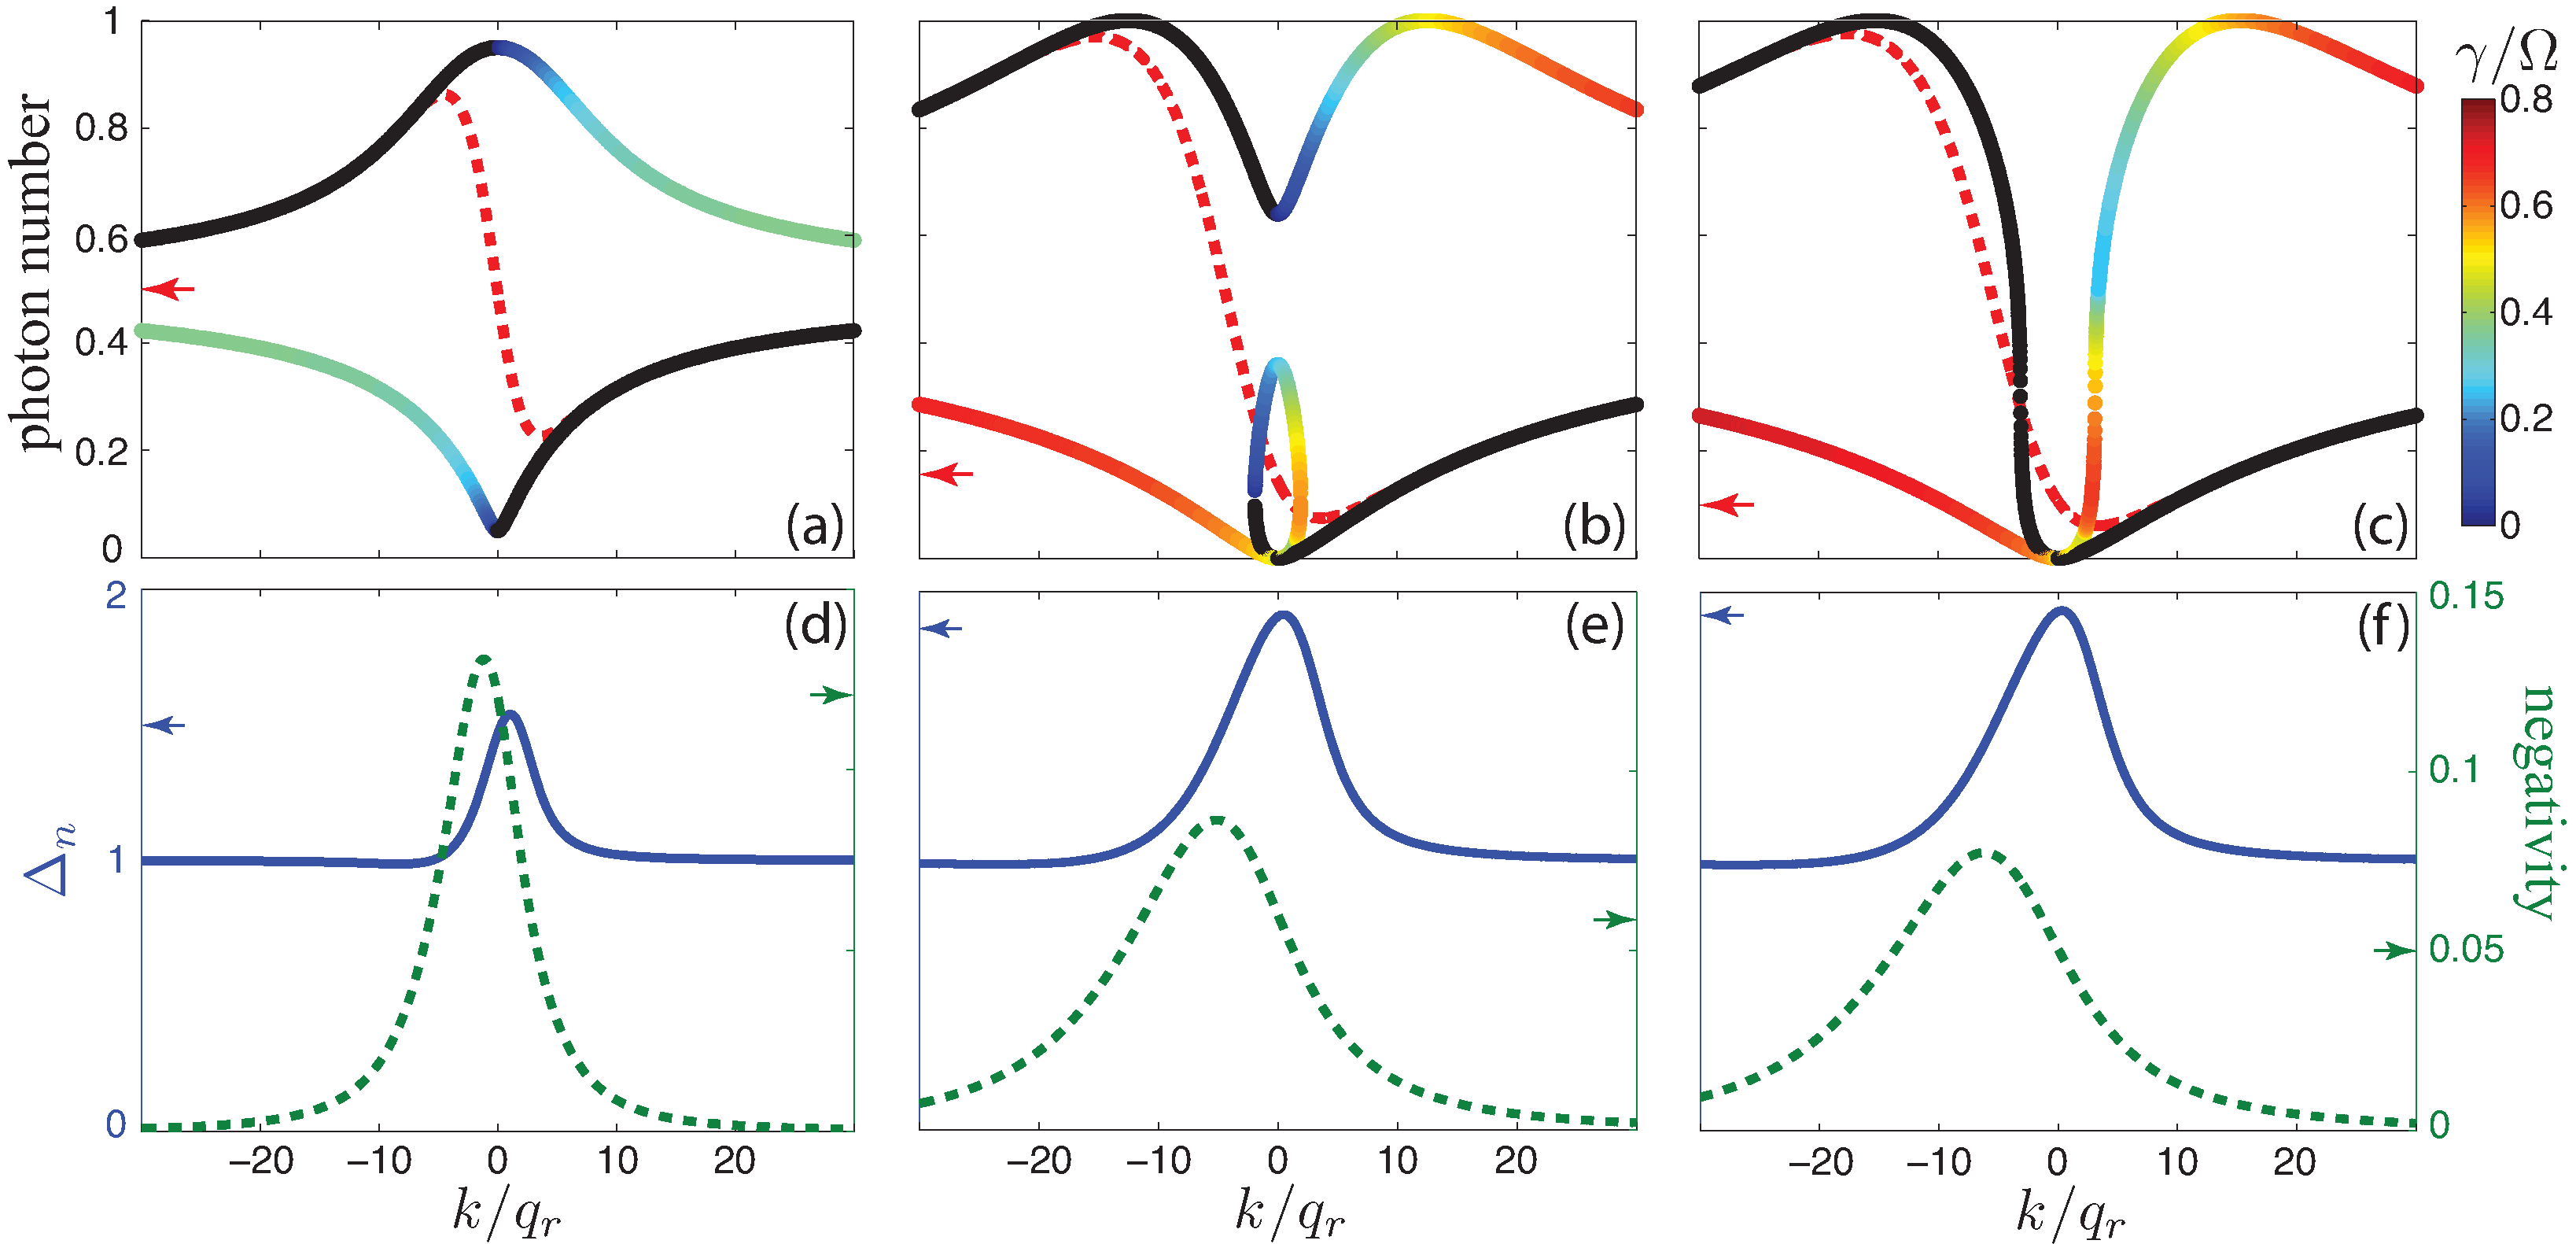
\includegraphics[width=\textwidth]{photon}
\caption{ Photon number comparison between semi-classical mean field result and full quantum mechanical master equation approach. From (a) to (c), $\Omega = 3\kappa,\quad 5.6\kappa,\quad 6\kappa$ and colorbar represents the renormalized decay rate $\gamma/\Omega$ of unstable states and red dashed lines are master equation solutions. Figure (d) to (f) plots the corresponding photon number fluctuation (blue solid curve) and negativity (green dashed line). At the large $k_z$ limit, we found $\text{Tr}[\rho_\text{photon}n]$ asymtotes to semi-classical mean field result $|\langle c\rangle|^2$, which further matches stable branches according to mean field stability analysis.}
\label{photon}
\end{figure}

As we show in Fig.~\ref{photon}(a)-(c), we compare photon number obtained from semi-classical mean field theory with full quantum master equation result. With increasing magnitude of $\Omega$, we sweep over regions with only two real roots, four real roots and only one double root (at $\epsilon=0$) to the mean field solution of Eq.~\ref{generalquarticEq}. We can further perform dynamical analysis \cite{cavitySOC} to pinpoint stable and unstable branches of the semi-classical solution. For unstable states, we use colorbar to denote the renormalized decay rate $\gamma/\Omega$ where $\gamma$ refers to the largest real eigenvalue of perturbed dynamical equation \cite{cavitySOC}. We found for any set of parameters and given $k_z$ value, we always have dynamically stable and unstable branches, regardless whether there is loop or not. This is rather surprising since it shows that the cavity back-action completely modifies the system's stability properties. For comparison, with the same parameter sets, we start from quantum master equation Eq.~\ref{EOMrho} and obtain steady state solution of density operator, and compute expectation value of photon number operator by tracing over the product, i.e. $\langle n\rangle=\text{Tr}[\rho n]$. We found, remarkably, in Fir.~\ref{photon} that $\text{Tr}[\rho n]$ recovers $|\langle c\rangle|^2$ value in dynamically stable branches, to a great extent. Several observations are in order. 
This agreement, first of all, further validates our previous semi-classical mean field treatment \cite{cavitySOC}. 
Second, at large $|k_z|$ value, master equation solution asymptotically collapes onto mean field solution, which can be complementarily understood from photon number fluctuation's behavior. From the definition of $\frac{\langle(\Delta n)^{2}\rangle}{\langle n\rangle}=\frac{\langle n^{2}\rangle-\langle n\rangle^{2}}{\langle n\rangle}$, we found the renormalized fluctuation magnitude degrades to unit one in this limit, where photon statistics is best modeled by the coherent state (Poissonian statistics) and atom's back-action {\em onto} photon becomes negligibly small. 
In order to further quantitatively characterize atom-photon feedback, we invoke the easily computable entanglement measure for mixed-state, the so-called negativity \cite{negativity}, defined as $\mathcal{N}(\rho)=\frac{||\rho^{T_A}||_1-1}{2}$, where $||\rho^{T_A}||_1$ denotes the trace norm of partial transpose of density operator with respect to atom party (the same is true for photon party). Density matrix $\rho$ itself gives all positive definite eigenvalues and thus the trace norm $||\rho||_1=\text{Tr}[\sqrt{\rho^\dagger\rho}]=\text{Tr}[\rho]=1$. Although the partial transpose $\rho^{T_A}$ still satisfies $\text{Tr}[\rho^{T_A}]=1$, it does not necessarily guarantee positive definiteness in eigenvalues. The trace norm is written generally as $||\rho^{T_A}||_1=1+2\sum_i|\mu_i|$ where we have denoted negative eigenvalues as $\mu_i<0$. Thus, by definition, the negativity $\mathcal{N}(\rho)$ is equal to $\sum_i|\mu_i|$ 
%-- the absolute sum of negative eigenvalues $\mu_i$ of $\rho^{T_A}$
, which measures by how much $\rho^{T_A}$ fails to be positive definite. An immediate consequence for any separable (unentangled) state $\rho_s$ is that $\mathcal{N}(\rho_s)=0$, while for unseparable mixed state, $\mathcal{N}(\rho)$ is believed to be a good entanglement measure. In Fig.~\ref{photon}(d)-(f), we plot negativity side by side with fluctuation for different $\Omega$ values. Despite the fact the two curves' peak centers at different $k_z$ value, one could still conclude that when atom and photon field is more entangled, photon number distribution deviates further away from Poissonian distribution. 
Third, there are regions where renormalized fluctuation is smaller than one, e.g. in Fig.~\ref{photon}(d) at small negative $k_z$ value,  $\frac{\langle(\Delta n)^{2}\rangle}{\langle n\rangle} \sim 0.95$, which implies sub-Poissonian photon number distribution as a signiture of system being genuinely non-classical. For the majority part, we have $\frac{\langle(\Delta n)^{2}\rangle}{\langle n\rangle}>1$ (super-Poissonian distribution), which leads to bunched spacing according to the statistics, i.e. more thermal like. In other words, ``slow'' atomic states have larger probabilities of back scattering cavity photon and photon field thus becomes more entangled and behaves like a source of chaotic light. It can be shown by the application of Cauchy-Schwarz inequality, the fluctuation term would have to be greater or equal to one, if we have a positive definite probability distribution for photon number. But it seems in our system, the photon number probability does not necessarily has to be greater than zero. ({\color{red} we can perhaps straightforwardly demonstrate this by plotting $p(n)=\langle n|\hat{\rho}_{\text{photon}}|n\rangle$ where $\hat{\rho}_{\text{photon}}$ is the reduced density matrix for photon by tracing over atomic degrees of freedom in total density opeartor, i.e. $\rho_{\text{photon}}=\text{Tr}_{\text{atom}}[\rho]$. For coherent light, $p_{\text{coh}}(n)=\frac{\langle n\rangle^{n}}{n!}e^{-\langle n\rangle}$; and for thermal light, $p_{\text{th}}(n)=\frac{1}{1+\langle n\rangle}(\frac{\langle n\rangle}{1+\langle n\rangle})^{n}$. We have found small pumping rate $\varepsilon_p$ gives better fit of $p(n)$ to  $p_{\text{th}}(n)$ and for large value of $\varepsilon_p$, $p(n)$ is closer to $p_{\text{coh}}(n)$.})

%After we have the steady state solution of total system's density operator, we can compute expectation value of photon number operator by tracing over the product, i.e. $\langle n\rangle=\text{Tr}[\rho n]=\rho_{nn}^{\uparrow\uparrow}+\rho_{nn}^{\downarrow\downarrow}$ and  photon number fluctuation $\frac{\langle(\Delta n)^{2}\rangle}{\langle n\rangle}=\frac{\langle n^{2}\rangle-\langle n\rangle^{2}}{\langle n\rangle}$. 
%As we show in Fig.~\ref{photon}, $\text{Tr}[\rho n]$ deviates from $|\langle c\rangle|^2$ at small $|k_z|$ value, where normalized fluctuation term is larger than one (super-Poissonian distribution). This mean cavity photon prefers to have bunched spacing according to the statistics, i.e. more thermal like. In other words, ``slow'' atomic states have larger probabilities of back scattering cavity photon and photon field thus becomes more entangled and behaves like a source of chaotic light.
% {\color{red} better interpretation?} 
%However, when we are in the large limit of  $|k_z|$, quantum results asymtopically approaches semi-classical mean field solution, while fluctuation magnitude uniformly degrades to unit one. This is the limiting case where photon statistics is best modeled by the coherent state (Poissonian statistics), where atom's back-action {\em onto} photon becomes negligibly small. And, semi-classical mean field theory agrees with quantum master solution in this limit. 
% {\color{red} better interpretation?}

%We can also consider the probability of finding $n$ photon, defined as $p(n)=\langle n|\hat{\rho}_{\text{photon}}|n\rangle$ where $\hat{\rho}_{\text{photon}}$ is the reduced density matrix for photon by tracing over atomic degrees of freedom in total density opeartor, i.e. $\rho_{\text{photon}}=\text{Tr}_{\text{atom}}[\rho]$. For coherent light, $p_{\text{coh}}(n)=\frac{\langle n\rangle^{n}}{n!}e^{-\langle n\rangle}$; and for thermal light, $p_{\text{th}}(n)=\frac{1}{1+\langle n\rangle}(\frac{\langle n\rangle}{1+\langle n\rangle})^{n}$. We have found small pumping rate $\varepsilon_p$ gives better fit of $p(n)$ to  $p_{\text{th}}(n)$ and for large value of $\varepsilon_p$, $p(n)$ is closer to $p_{\text{coh}}(n)$. Since we always have a positive definite probability distribution for photon number, the fluctuation term would have to be greater or equal to one, which can be shown by an application of the Cauchy-Schwarz inequality.
 %{\color{red} would there be any region of parameter that gives sub-Possonian field, that are genuinely non-classical feature of quantum optics? Negative Mandel Q parameter, second order intensity correlation function etc.}


%[{\color{red} Rewrite it, simplify it and highlight it.}] Negativity for mixed state is defined as $\mathcal{N}(\rho)=\frac{||\rho^{T_{atom}}||_{1}-1}{2}=\frac{\left(\sum\text{eig}[\rho^{T_{\text{atom}}}]\right)-1}{2}=\sum_{i}\frac{|\lambda_{i}|-\lambda_{i}}{2}$ where $\lambda_{i}$ are all the eigenvalues of $\rho^{T_{atom}}$. Namely, nagativity is the absolute sum of negative eigenvalues of $\rho^{T_{atom}}$, which vanishes for unentangled states. Also, $\rho^{T_{atom}}$ stands for partial transpose of density matrix with respect to atom party, $\rho^{T_{atom}}=\left(\begin{array}{cc} [\rho_{mn}^{\uparrow\uparrow}]^{T} & [\rho_{mn}^{\uparrow\downarrow}]^{T}\\ {}[\rho_{mn}^{\downarrow\uparrow}]^{T} & [\rho_{mn}^{\downarrow\downarrow}]^{T}\end{array}\right)$.




\section{Conclusions} \label{conclusion}

We have studied spin-orbit coupled cold atoms inside a ring cavity system, and found interesting XXX.

\acknowledgments{Acknowledgments}
We acknowledge discussions with Zhengwei Zhou and XXX. H.P. is supported by the NSF and Welch Foundation (Grant No. C-1669 XXX);
\authorcontributions{Author Contributions}
H.P. conceived the idea of the project, L.D. and C. Z. explored the theoretical and numerical aspects of the physics. All authors contributed to writing and revising the manuscript and participated in the discussions about this work.
\conflictofinterests{Conflicts of Interest}
The authors declare no conflict of interest. 

%=================================================================
% References: Variant A
%=================================================================
% Back Matter (References and Notes)
%----------------------------------------------------------
% Style and layout of the references
% Reference 1
% \bibitem{ref-journal}
% Lastname, F.; Author, T. The title of the cited article. {\em Journal Abbreviation} {\bf 2008}, {\em 10}, 142-149
\bibliographystyle{mdpi}
\makeatletter
\renewcommand\@biblabel[1]{#1. }
\makeatother
\begin{thebibliography}{999} % if there are less than 10 entries, enter a one digit number
\bibitem{BEC1}
Anderson, M. H., J. R. Ensher, M. R. Matthews, C. E. Wieman, and E. A. Cornell, {\em Science} {\bf 1995}, {\em 269}, 198.
\bibitem{BEC2}
Bradley, C. C., C. A. Sackett, J. J. Tollett, and R. G. Hulet, {\em Phys. Rev. Lett.} {\bf 1995}, {\em 75}, 1687.
\bibitem{BEC3}
Davis, K. B., M.-O. Mewes, M. R. Andrews, N. J. van Druten, D. S. Durfee, D. M. Kurn, and W. Ketterle, {\em Phys. Rev. Lett.} {\bf 1995}, {\em 75}, 3969.
\bibitem{Fermi1}
DeMarco, B., and D. D. Jin, {\em Science} {\bf 1999}, {\em 285}, 1703.
\bibitem{Fermi2}
Truscott, A., K. Strecker, W. McAlexander, G. Partridge, and R. G. Hulet, {\em Science} {\bf 2001}, {\em 291}, 2570.
\bibitem{Fermi3}
Schreck, F., L. Khaykovich, K. L. Corwin, G. Ferrari, T. Bourdel, J. Cubizolles, and C. Salomon, {\em Phys. Rev. Lett.} {\bf 2001} {\em 87}, 080403.
\bibitem{Bloch1}
Bloch, I., {\em Nature Physics} {\bf 2005}, {\em 1} 23. 
\bibitem{Bloch2}
Bloch I. and M. Greiner, {\em Adv. At. Mol. Opt. Phys.} {\bf 2005}, {\em 52} 1.
\bibitem{BH1}
Jaksch, D., C. Bruder, J. I. Cirac, C. W. Gardiner, and P. Zoller, {\em Phys. Rev. Lett.} {\bf 1998}, {\em 81}, 3108.
\bibitem{BH2}
W. Zwerger, {\em J. Opt. B} {\bf 2003}, {\em 5}, 9.
\bibitem{Fermi4}
Chevy, F.;Salomon, C. Thermodynamics of Fermi Gases. In {\em The BCS-BEC Crossover and the Unitary Fermi Gas}; Zwerger, W.; Springer: Lecture Notes in Physics, Vol. 836, 2012; pp. 407-446.
\bibitem{Fermi5}
Ketterle, W.; Zwierlein, M. W., Making, probing and understanding ultracold Fermi gases. In {\em Ultra-cold Fermi Gases}; Inguscio, M., Ketterle, W., Salomon, C.; IOP Press:Proceedings of the International School of Physics ``Enrico Fermi'', 2007; pp.95-287.
\bibitem{cavity1}
Brennecke, F., Donner, T., Ritter, S., Bourdel, T., Kohl, M., and Esslinger, T., {\em Nature} {\bf 2007}, {\em 450} 268.
\bibitem{cavity2}
Colombe, Y., Steinmetz, T., Dubois, G., Linke, F., Hunger, D. and Reichel, J. {\em Nature} {\bf 2007}, {\em 450} 272.
\bibitem{cavity3}
Slama, S., Bux, S., Krenz, G., Zimmermann, C. and Courteille, Ph. W. {\em Phys. Rev. Lett.} {\bf 2007}, {\em 98} 053603.
\bibitem{cavity4}
J. M. Raimond, M. Brune, and S. Haroche, {\em Rev. Mod. Phys.} {\bf 2001}, {\em 73}, 565.
\bibitem{cavity5}
R. Miller, T. E. Northup, K. M. Birnbaum, A. Boca, A. D. Boozer, and H. J. Kimble, {\em J. Phys. B} {\bf 2005}, {\em 38}, S551.
\bibitem{cavity6}
H. Walther, B. T. H. Varcoe, B.-G. Englert, and T. Becker, {\em Rep. Prog. Phys.} {\bf 2006}, {\em 69}, 1325.
\bibitem{cavity7}
F. Brennecke, T. Donner, S. Ritter, T. Bourdel, M. Köhl, and T. Esslinger, {\em Nature} (London) {\bf 2007}, {\em 450}, 268.
\bibitem{cavity8}
Y. Colombe, T. Steinmetz, G. Dubois, F. Linke, D. Hunger, and J. Reichel, {\em Nature} (London) {\bf 2007}, {\em 450}, 272.
\bibitem{cavity9}
S. Slama, S. Bux, G. Krenz, C. Zimmermann, and Ph. W. Courteille, {\em Phys. Rev. Lett.} {\bf 2007}, {\em 98}, 053603.
\bibitem{cavity10}
D. Schmidt, H. Tomczyk, S. Slama, and C. Zimmermann, arXiv:1311.2156 (2013).
\bibitem{cavity11}
S. Gupta, K. L. Moore, K. W. Murch, and D. M. Stamper-Kurn, {\em Phys. Rev. Lett.} {\bf 2007}, {\em 99}, 213601.
\bibitem{cavity12}
M. Lewenstein, A. Sanpera, V. Ahufinger, B. Damski, A. Sen De, and U. Sen, {\em Adv. Phys.} {\bf 2007}, {\em 56}, 243.
\bibitem{cavity13}
I. B. Mekhov and H. Ritsch, {\em J. Phys. B} {\bf 2012}, {\em 45}, 102001.
\bibitem{soc1}
Y.-J. Lin, K. Jimenez-Garcia, and I. B. Spielman, {\em Nature} (London) {\bf 2011}, {\em 471}, 83.
\bibitem{soc2}
Y.-J. Lin, R. L. Compton, K. Jimenez-Garcia, W. D. Phillips, J. V. Porto, and I. B. Spielman, {\em Nat. Phys.} {\bf 2011}, {\em 7}, 531.
\bibitem{soc3}
P. Wang, Z.-Q. Yu, Z. Fu, J. Miao, L. Huang, S. Chai, H. Zhai, and J. Zhang, {\em Phys. Rev. Lett.} {\bf 2012}, {\em 109}, 095301.
\bibitem{soc4}
L. W. Cheuk, A. T. Sommer, Z. Hadzibabic, T. Yefsah, W. S. Bakr, and M. W. Zwierlein, {\em Phys. Rev. Lett.} {\bf 2012}, {\em 109}, 095302.
\bibitem{socVictor}
V Galitski, IB Spielman, {\em Nature} {\bf 2013}, {\em 494} 7435.
\bibitem{TI}
Hasan, M. Z., Kane, C. L. {\em Rev. Mod. Phys.} {\bf 2010}, {\em 82} 3045–3067.
\bibitem{MF}
Sau, J. D., Lutchyn, R. M., Tewari, S. and Sarma, Das, S. {\em Phys. Rev. Lett.} {\bf 2010}, {\em 104} 040502.
\bibitem{WF}
Burkov, A. A. and Balents, L.,  {\em Phys. Rev. Lett.} {\bf 2011}, {\em 107} 127205. 
\bibitem{SHE1}
Sinova, J., Cilcer, D., Niu, Q., Sinitsyn, N., Jungwirth, T., and MacDonald, A.,  {\em Phys. Rev. Lett.} {\bf 2004}, {\em 92} 126603.
\bibitem{SHE2}
Kato, Y. K., Myers, R. C., Gossard, A. C. and Awschalom, D. D.,  {\em Science} {\bf 2004}, {\em 306} 1910–1913.
\bibitem{cavitySOC}
Lin Dong, Lu Zhou, Biao Wu, B. Ramachandhran, and Han Pu, {\em Phys. Rev. A} {\bf 2014} {\em 89}, 011602(R).
\bibitem{L1}
Kossakowski, A. { Rep. Math. Phys.} {\bf 1972}, {\em 3} (4): 247.
\bibitem{L2}
Lindblad, G. {\em Commun. Math. Phys.} {\bf 1976}, {\em 48} (2): 119.
\bibitem{negativity}
Vidal, G., Werner, R. F., {\em Phys. Rev. A} {\bf 2002}, {\em 65} 032314.
% Reference 2
% \bibitem{ref-book}
% Lastname, F.F.; Author, T. The title of the cited contribution. In {\em The Book Title}; Editor, F., Meditor, A., Eds.; Publishing House: City, Country, 2007; pp. 32-58.
\end{thebibliography}
\end{document}

